% #############################################################################
% This is Chapter 3
% !TEX root = ../main.tex
% #############################################################################
% Change the Name of the Chapter i the following line
\fancychapter{System design and implementation}
\cleardoublepage
% The following line allows to ref this chapter
\label{chap:implement}
\section{Introduction} 

The main goal of this work is developing an end-user application for \ac{ET}, that uses blockchain as a payment method and contemporarily provides \ac{EF} through a low-cost and easy to use the system.


Taking into account lessons learned from previous studies in both areas of \ac{EFS} and \ac{P2P} \ac{ET}, the system was designed as a mobile application (developed for Android since it is open source).



Despite all participants in the field study aimed at testing the app are prosumers, \ac{PS} targets also consumers. Therefore, the motto while designing the application was “keep it simple”, that is to say, easy to use and understand for the wider audience possible (including people with a limited knowledge on energy).



\ac{PS} allows automated energy tradings between neighbors. It provides users with the opportunity to set the parameters for buying and/or selling energy, as well as to access and monitor data regarding their energy consumption, production (in case the user is a prosumer), and transactions.



The application is connected with \ac{PS} \ac{ETMS} that is responsible for managing users’ accounts, managing energy demand and offer, and providing data about the users’ overall energy consumption and production. Data are collected through a smart meter, installed in each household participating in the study, which measures production and consumption. The integration of IOTA technology will serve the purpose of carrying out the transactions between neighbors in a decentralized fashion.


\Cref{fig:ps} shows the architecture of the system. The grey arrows represent the regulated electricity network (the power grid*), which is managed by the local \ac{DSO} and is therefore independent of our system. Each household has its own solar PV system and BESS*. When PowerShare \ac{ETMS} find a match between energy demand and offer, it automatically starts the transaction, which is then paid using IOTA node as a service.  

\begin{figure}[h]
\centering
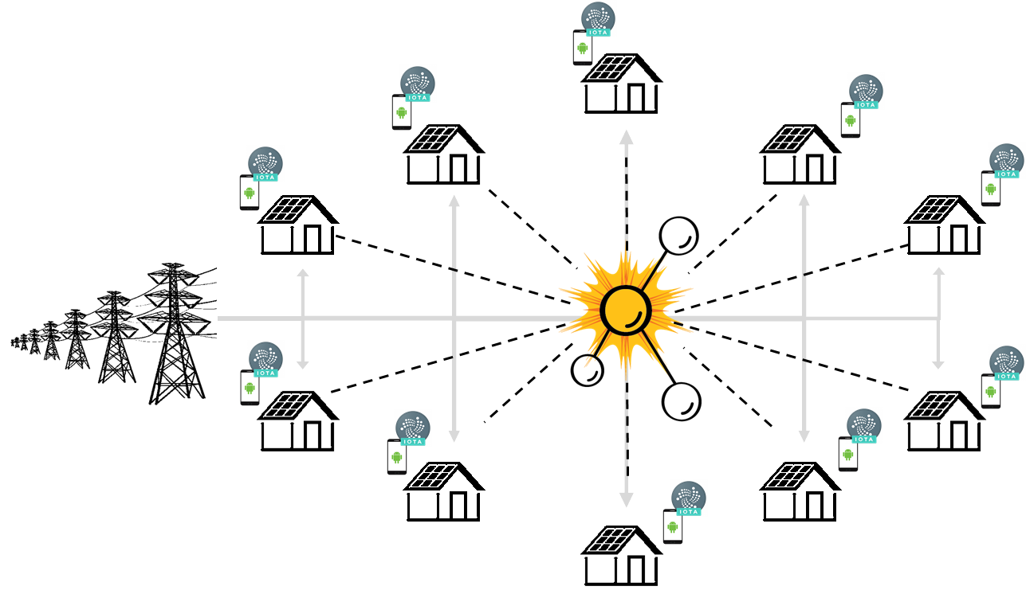
\includegraphics[width=1.0\textwidth]{./Images/ps}
\caption{Power Share system illustration}
\label{fig:ps}
\end{figure}


The following sections provide a detailed description of both front- and back-end of the application, as well as of the integration of IOTA technology. Requirements and constraints that led to the final solution are also presented. 

\section{Power Share Application}


This section describes all the process of design and implementation of the front-end of the \ac{PS} mobile application.



\subsection{Design}


Once the requirements and main goal  were defined, we started designing the front-end of the app.  During an initial brainstorming, we wrote down onto sticky notes a set of aspects (found after reviewing the literature on \ac{EFS} and \ac{ET} and analyzing outcomes of existing projects) related to:

\begin{itemize}
    \item Users needs;
    \item Obstacles to adoption;
    \item Limitations of both systems;
    \item Insights.
\end{itemize}


Then, the stick notes were sorted into groups through an affinity diagram, looking for relationships and patterns. By following this process, the following main sections/features of the app were identified:



\begin{itemize}
    \item \textbf{Home:} showing current consumption and production. Real--time feedback is indeed often defined as a requirement by users of EFS and helps them better understand the link between an action and its effect (e.g. peak consumption after turning on the hair dryer);
    \item \textbf{Settings:}through which the user can define the criteria to buy/sell energy;
    \item {Historical:} provides the user’s consumption/production data over time (which has been found to be one of the most appreciated features by EFS users and, at the same time, provides a set of information that could be of great help in identifying the best criteria to buy/sell energy);
    \item \textbf{Transactions:} showing a list of all transactions made by the user;
    \item \textbf{Ranking:} since social comparison has been proven to an effective leverage to foster behavioral change, this section shows to the user how his consumption of renewable energy compares to the other users.
\end{itemize}


The navigation tree and some basic requirements of \ac{UI}/\ac{UX} were also defined. First of all, the \ac{UI} has to be simple (but not simplistic), user-friendly, clear and appealing. Data provided through the app must be detailed in order to avoid misunderstandings but, contemporarily, limited to the most relevant ones in order to avoid information overload. The “setting” should be designed targeting those users that have a limited knowledge of energy. Also, negative feedback should be avoided.


The resulting wire frames were subjected to a quick heuristic evaluation of layout elements, function, and flow, after which possible bottlenecks were identified and removed. Then, a low-fidelity prototype was realized and tested with a small group of researchers and students from the Madeira Interactive Technologies Institute, all with a limited knowledge of energy.
Participants in the pilot test performed the following tasks:
\begin{enumerate}
    \item Registration of a new account. All participants concluded that task successfully. Since the registration process requires users to input some information about their \ac{PV} installation (in prosumers mode) and contract with the energy supplier, the \ac{UI} included tips to help users filling out the input fields. Nevertheless, some of the participants did not see them immediately, suggesting us to make them more noticeable. 
    \item Modify account settings. Again, all users complete the task, but some of them selected first the “trading settings” feature, suggesting the need to make the purpose of each section more clear by rethinking carefully both labels and icons.
    \item Configure the parameters to buy and sell energy. The main issue here was that users did not understand that there were mandatory (e.g. set a price) and not mandatory fields (e.g. define specific time frame when buying/selling energy). To address this issue sub headers were added as shown in \cref{fig:ps1}.
    \item Check the list of transactions carried out. Some users select “Histórico”. Such a mistake was due to the icons design, which turned out to be misleading.
    \item Check historical production/consumption data. All participants concluded that task successfully and the visualization designed (a stacked bar graph) resulted clear to everyone.
    \item Check current energy usage (Home). All participants concluded that task successfully.
    \item Check your achievements (Rankings). All participants concluded that task successfully.
\end{enumerate}


\begin{figure}[h]
\centering
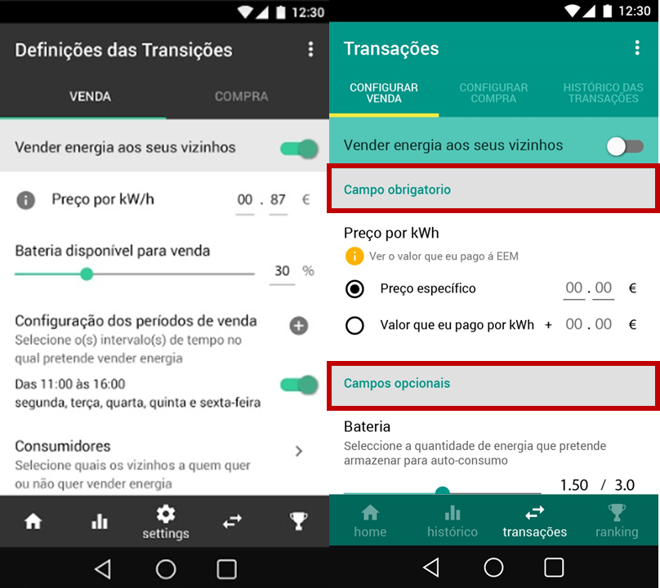
\includegraphics[width=0.7\textwidth]{./Images/ps1}
\caption{Sell settings layout before and after heuristic evaluation}
\label{fig:ps1}
\end{figure}


At the end of each user test, participants were also asked for comments and opinion about their experience. Through their feedback other two issues were identified:

\begin{itemize}
    \item Many participants said that they didn't really get why the list of transactions and transactions setting were separated, thus we decided to combine them in a single section \cref{fig:ps2}.
    \item Some participants raised possible privacy concerns about sharing with the community information about the amount of renewable energy they used. For this reason, we decided to make it possible for them to not share this information.
\end{itemize}


\begin{figure}[h]
\centering
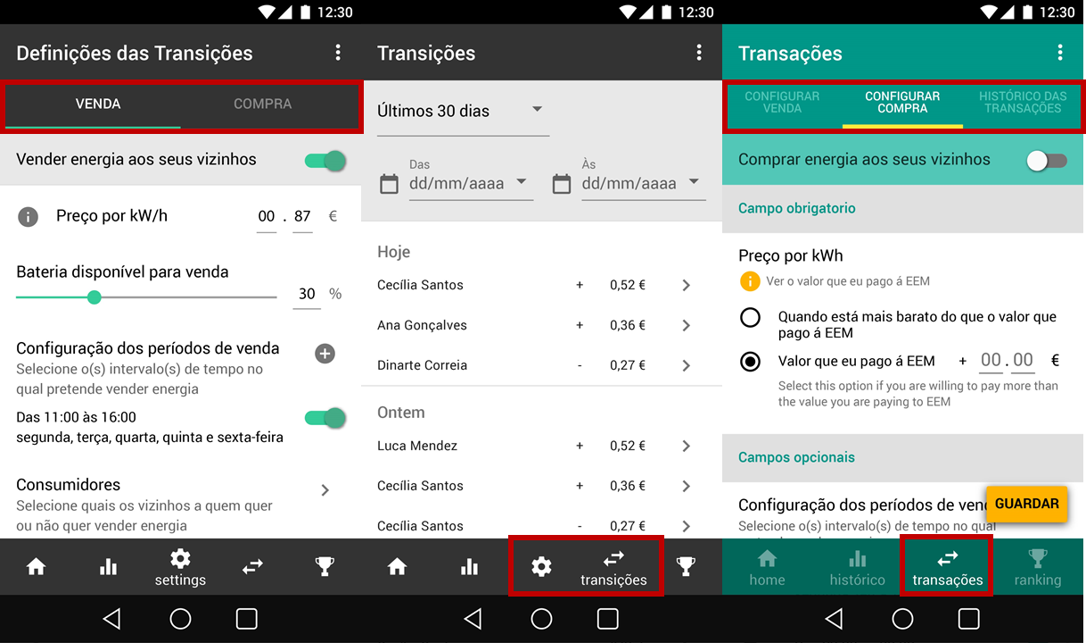
\includegraphics[width=1\textwidth]{./Images/ps2}
\caption{Sell settings/historical tradings layout before and after heuristic evaluation}
\label{fig:ps2}
\end{figure}

On the basis of the above-mentioned results, another low-fidelity prototype was designed and tested with different subjects. The changes made resulted resulted in the improvement of users performance allowing us to start designing the \ac{UI} mockup.

In terms of flow, we tried to keep the registration process as quick as possible. Creating a new account requires three main steps (see \cref{fig:ps3}):
\begin{enumerate}
    \item Defining users credentials: first and last name, email address and password;
    \item Input some basic information about the contract with the energy provider: voltage range, contracted power, electricity tariff and cycle (only if applicable). Here, according to the feedback from the pilot test, the information buttons showing where to find such information on the electricity bill were emphasized.
    \item Defining user typology (consumer or prosumer). In case the user registers as a prosumer, I’ll be asked to input further information concerning solar panels and battery owned.
\end{enumerate}


Before finishing the registration, users receive an IOTA seed\footnote{In a real case the user could use a seed if he already have one or generate one in the app. For this study we create the accounts and pre-charge them and only ask the user to set out a password to cipher the seed and store it.}, which gives them access to their IOTA account. Users are thus asked to set a password for that seed.
During the registration process, the user is asked to allow or not the app to share within the community the share of RES in his/her overall energy consumption. Whatever choice they make, a dialog informs them that they can always provide or deny permission anytime, by accessing their account settings. In addition, at the end of the registration, the user is provided with the opportunity to select the “automatic settings” for the buying and selling criteria. By selecting the automatic settings, users will immediately start trading energy while, if they choose the manual mode, they have to set the buying and selling criteria in "transactions" before being able to trade. Also, in this case, users are informed that they can modify this choice at any time through their account settings.

\begin{figure}[h]
\centering
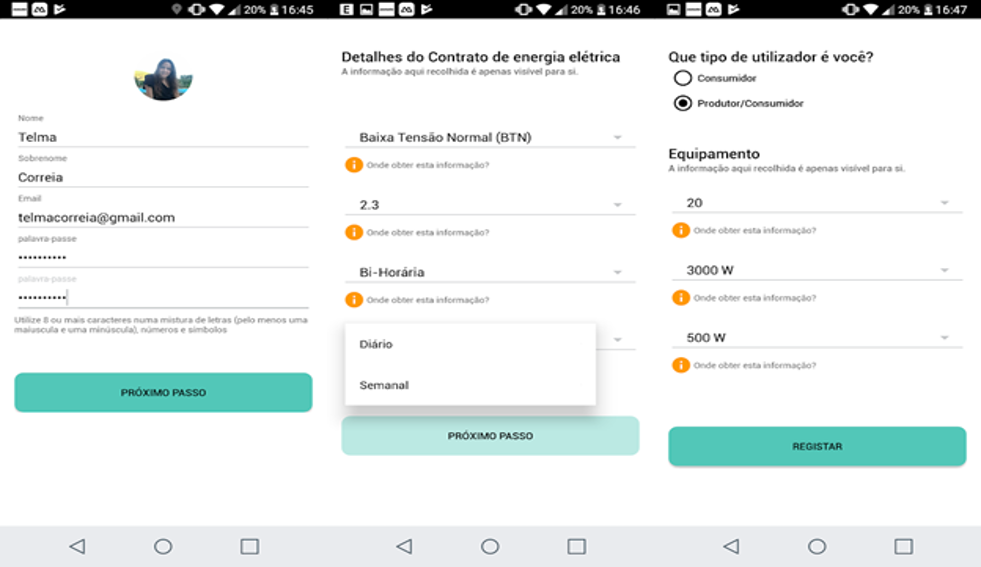
\includegraphics[width=1\textwidth]{./Images/ps3}
\caption{Registration layouts}
\label{fig:ps3}
\end{figure}


Once the user is finally registered, (s)he can access the four main feature of the app \cref{fig:ps4}.


\begin{figure}[h]
\centering
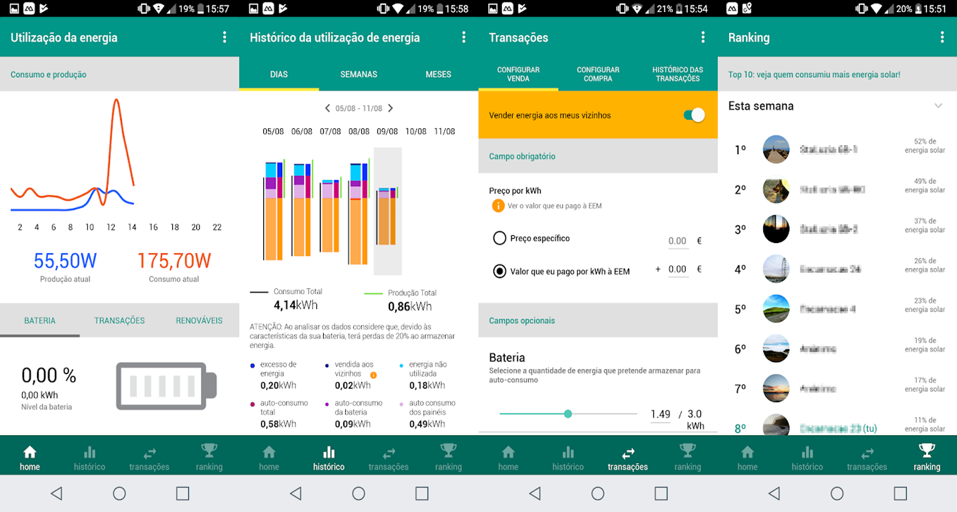
\includegraphics[width=1\textwidth]{./Images/ps4}
\caption{Main Power Share menus}
\label{fig:ps4}
\end{figure}


\textbf{Home:}
The home provides information about (\cref{fig:ps4}, 1st on the left):
\begin{itemize}
    \item current production and consumption (line chart on the top of the screen);
    \item the battery status (amount of energy stored) (\cref{fig:ps5}, 1st on the left);
    \item a summary of transactions carried out that day. Such information is presented through a heat map so to help the user identify at a glance at what time of the day (s)he buys and sell more energy. Further details about each transaction can be accessed by selecting the green arrow on the top of the heat map (\cref{fig:ps5}, the image in the middle);
    \item the share of RES in the user weekly energy consumption (\cref{fig:ps5}, 1st on the right): here the user can quickly check how much RES is using in the current week (donut chart) and how is (s)he doing in comparison to the other users (ranging from “very good”, represented by a smiling face, to “you should do better”, represented by a frowning face). The comparison with other users is always coupled with an encouraging sentence, in order to avoid a negative feedback. Data are updated every minute.
\end{itemize}

\begin{figure}[h]
\centering
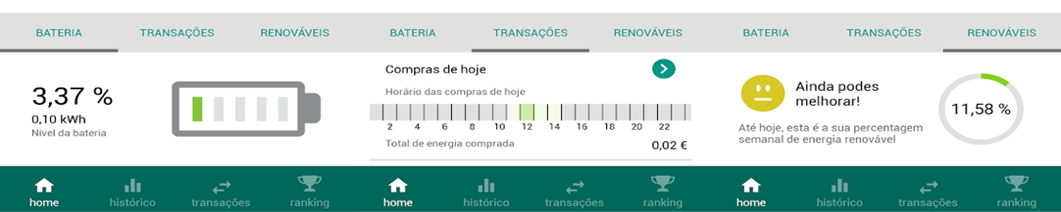
\includegraphics[width=1\textwidth]{./Images/ps5}
\caption{Home menu tabs}
\label{fig:ps5}
\end{figure}
\textbf{Histórico:} (\cref{fig:ps4}, 2nd on the left)
Through this feature, users can access their own past consumption and production data, with three levels of temporal granularity (days, weeks, months). The information is illustrated through a stacked bars graph as well as a table (on the bottom of the graph, which also serves as a legend to the graph). Not only overall production and consumption are presented, but also their respective breakdown (e.g. consumption is divided in energy bought from the supplier, from neighbours, and from self-consumption), so the user can leverage this information to modify his/her buying and selling criteria (if needed).
\Cref{fig:ps6} represents an example the information presented to users in the “histórico”.

\begin{figure}[h]
\centering
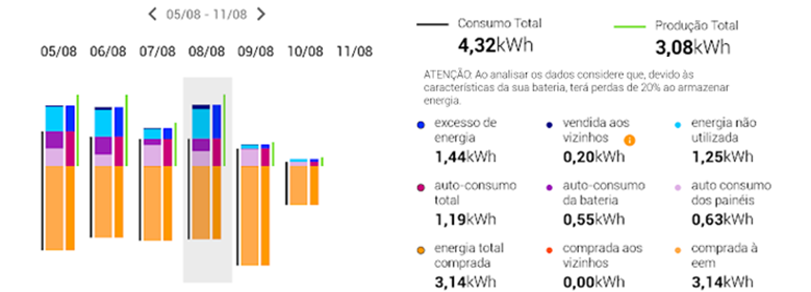
\includegraphics[width=0.7\textwidth]{./Images/ps6}
\caption{Historical daily graph}
\label{fig:ps6}
\end{figure}


As shown in \cref{fig:ps7}, for each time frame (a day, a week, or a month), the user is provided with the following information:
Energy surplus (a) and its breakdown: surplus sold to neighbours (a1) and surplus stored in the battery (a2);
Self-consumption (b), divided in direct consumption (b1) - from solar panels - and consumption from the battery (b2). This, in order to help users understanding the percentage of total battery capacity needed to fulfill their energy need and, consequently, the amount of energy they can sell to neighbours.
Energy purchased (c) and its breakdown: purchased from \ac{EEM} (c1) and from neighbours (c2).
In addition, to help users compare their total production (d1) and consumption (d2), two small line have been added to the graph.

\begin{figure}[h]
\centering
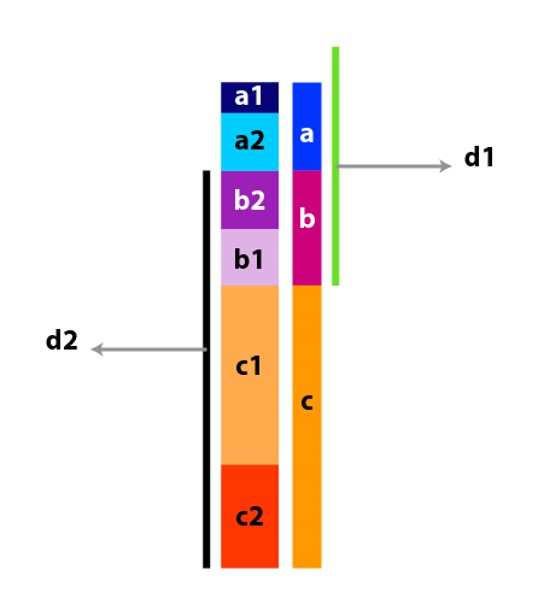
\includegraphics[width=0.5\textwidth]{./Images/ps7}
\caption{Graphical explanation for each column}
\label{fig:ps7}
\end{figure}


As shown in  \cref{fig:ps6}, the graph is always combined with a table which serves as a legend for the graph itself and provides detailed information about energy use so to prevent the user to misinterpret the visualization or, even worst, think there is something wrong with the data. For example, a user could get confused noticing that total production (green line) always exceeds the sum of “energy surplus” and “self-consumption”. An alert in the table explains that this is due to the fact that when using a Battery Energy Storage System there is always a loss of energy (about 20\%)\footnote{This is better explained in the \ref{psetms}}. In addition, in case the energy sold to neighbours and/or stored in the battery exceeds the “energy surplus” of that day/week/month, through an info button the user is provided with an explanation for that - i.e. there was still energy stored in the battery from the previous day/week/month.
Last but not least, every time the battery is full, an alert button will appear (\cref{fig:ps8}). If the user presses it, a dialog opens up and warns him that he is “wasting” his production because cannot store energy in the battery anymore.


\begin{figure}[h]
\centering
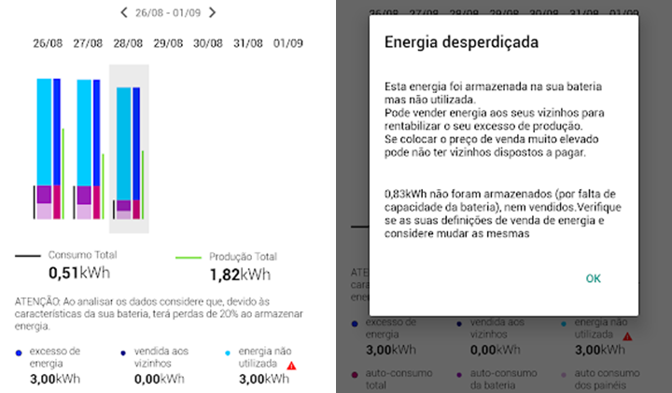
\includegraphics[width=0.7\textwidth]{./Images/ps8}
\caption{Example of wasted energy alert}
\label{fig:ps8}
\end{figure}


\textbf{ Transações: buying/selling criteria:} (\cref{fig:ps9})

This section is divided into three main sub-sections: 1) manual definition of criteria for selling energy; 2) manual definition of criteria for buying energy; 3) list of all transactions performed.
The core of the application is the manual definition of buying/selling criteria. The only mandatory field here is “price for kWh”. The user is indeed required to define at what price (s)he is willing to buy as well as sell energy. In both cases, two are the possible options: 1) a fixed price (“maximum” fixed price in the case of buying criteria); 2) a price tied to the cost of energy he/she buys from the electricity company (in the case of Madeira it is \ac{EEM}). The latter option is targeted to consumers that are subjected to dynamic pricing (i.e. have a bi-horária or tri-horária tariff), thus pay energy at different prices at different times of the day. Concerning “energy selling”, such price could be equal or bigger to the cost of energy (s)he buys from \ac{EEM} at a given moment while, regarding “energy buying”, the users set a maximum price which could be equal or lower than the cost of energy bought from \ac{EEM} at a given time. Results from the \ac{SINAIS} project revealed that many consumers are not aware of the cost of energy and, sometimes, don’t even know their own tariff. Therefore, in order to support users in defining the price for the energy they are buying and/or selling, an “information button” was added, which opens up a dialog providing information about the user’s tariff and relative energy prices. 
In both “energy buying” and “energy selling” sections there are then the following optional criteria:
\begin{itemize}
    \item Select one or more specific time frames for buying and/or selling energy;
    \item Select people you want to trade with (buy from and sell to) among the users in the community. Every time someone joins the community, all users that decided to trade only with specific people receive a notification (\cref{fig:ps10}), so they can include or not the new user among them. 
    \item Save part of the overall storing capacity of your battery for self-consumption only (this criterion is available only for energy selling). 
\end{itemize}


\begin{figure}[h]
\centering
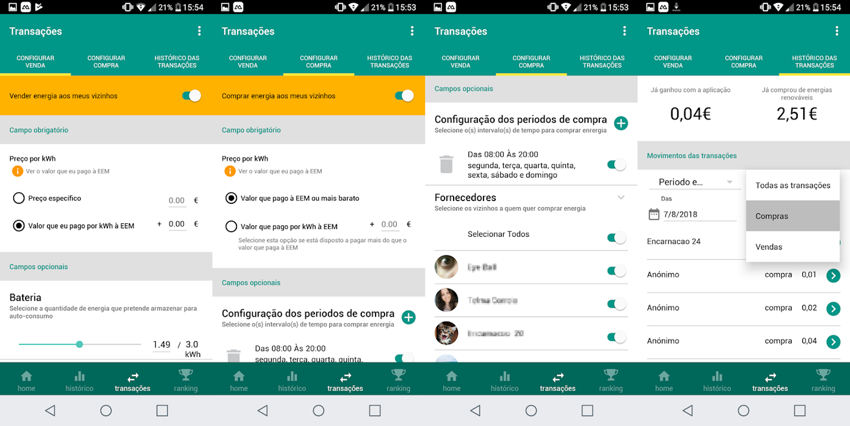
\includegraphics[width=1\textwidth]{./Images/ps9}
\caption{Power Share: Sell/Buy Settings layouts}
\label{fig:ps9}
\end{figure}

If users do not set any of the above mentioned optional criteria, (s)he will be notified that, for instance, (s)he is going to buy energy from anyone and at any time. Once all the parameters are defined, the user can start trading energy by using the slider on the top of the screen. In the same way, the user can momentarily disable the trading while keeping his/her settings as such.
The list of transaction (\cref{fig:ps9}, last one from left to right) users can quickly see their total earnings/expenses and all transactions (s)he carried out.  The list could be filtered by date range and/or by type of transaction (buying or selling). Further details about each transaction are also provided.  



\textbf{Ranking}
Here it is presented the rating for top 10 users (among those who allowed the app to display such information) with the biggest share of RES consumption. The current user place appears always in the list even if (s)he is not in the top 10.

An overflow menu is placed in the top app bar, which allows the user to access some secondary features:
\begin{itemize}
    \item Account settings;
    \item Privacy Policy;
    \item IOTA wallet.
\end{itemize}


\begin{figure}[h]
\centering
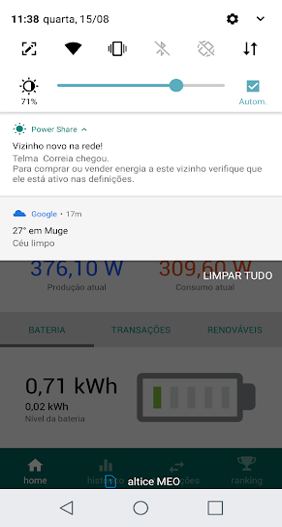
\includegraphics[width=0.3\textwidth]{./Images/ps10}
\caption{New neighbour notification}
\label{fig:ps10}
\end{figure}

\subsection{Implementation}

The rationale behind a developing a mobile application for android is that it is  more versatile and accessible since android is an open source system. In order for the app to quickly respond to changes, the Model View-ViewModel (MVVM) design pattern was adopted. This pattern has 3 main layers and lots of advantages:
\begin{itemize}
    \item \textbf{The View:} it basically consists in the layout of each screen. The View is responsible for informing the View Model Layer about the user’s actions;
    \item \textbf{The View Model} takes care of relevant data for the View layer;
    \item \textbf{The Data Model}, which is a data source abstraction. The View Model Layer works with the Data Model to get and save the data. 
\end{itemize}

A clear advantage of this pattern is the abstraction between the domain logic and presentation layer. It also makes the code easier to maintain, test and extend. \ac{MVVM} was used together with RxJava, a Java implementation of Reactive Extensions\footnote{\url{https://github.com/ReactiveX/RxJava/wiki}}, which consists in a library for composing asynchronous and event-based programs by using observable sequences.
Other relevant libraries used to develop the app are listed below:
\begin{itemize}
    \item Dagger: a fully static, compile-time dependency injection framework for Java and Android\footnote{\url{https://google.github.io/dagger/}};
    \item Retrofit\footnote{\url{http://square.github.io/retrofit/}}: a library for HTTP-client connections;
    \item MPAndroidChart\footnote{\url{https://github.com/PhilJay/MPAndroidChart}}: Chart views for Android;
    \item Firebase\footnote{\url{https://console.firebase.google.com/}}: Cloud messaging (notifications);
    \item IOTA API\footnote{\url{ https://github.com/iotaledger/iota.lib.java}}: Java wrapper around IOTA.
\end{itemize}


The \ac{UI} was designed mainly for mobile phones, nevertheless, the layout is fully responsive so it perfectly adapts to tablets. The only requirements for the application to run is a mobile device running Android 4.4.2 or higher with \ac{API} level greater or equal to 19. 


The most crucial feature implemented for the purpose of this project is the IOTA payment. As explained before, each user is provided with a seed that gives him/her access to an IOTA account. Such seed needs to be securely stored.,  Therefore, the user is required to set a password for it (\cref{fig:ps11}, first image) and only then, the seed ciphered is stored in the server. For security reasons, the deciphered seed cannot be stored on the mobile device, consequently, payments cannot be fully automated and each time a user wants to access the wallet (“ver o meu saldo”), (s)he is asked for the password set. Once the password is inputted the seed is deciphered and can be used (the seed stays only deciphered in memory, is not stored deciphered in a persistent way) .


\begin{figure}[h]
\centering
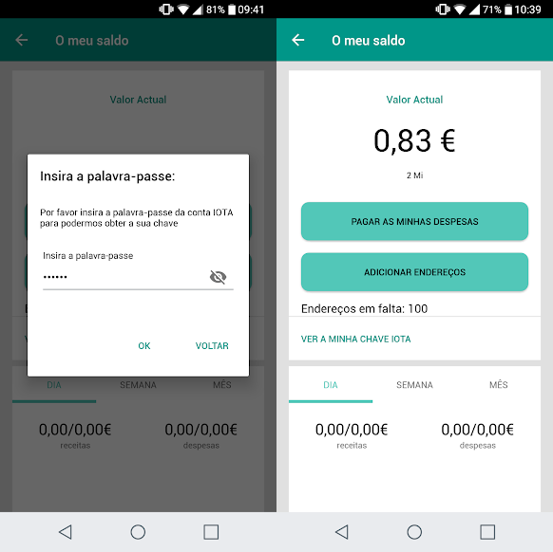
\includegraphics[width=0.3\textwidth]{./Images/ps11}
\caption{IOTA wallet in Power Share}
\label{fig:ps11}
\end{figure}

Through the wallet, users can check their account details (e.g.balance; daily, weekly and monthly incomes/outcomes).



The query for balance information could take a while to be executed, depending on IOTA node state. The same might happen when the user generates  new destination addresses (see \cref{seciotatech}). With this respect, it should be pointed out that each transaction carried out by the user as seller requires a new address. When (s)he runs out of addresses, receives a push notification and an email asking to generate new addresses. To make the payment, the user has to press the “pagar as minhas despesas” button. If the user has not enough balance, the payment will be rejected by the node. It is, of course,  user responsibility to have enough balance to keep trading.


Since the application has no database, SharedPreferences is used to persistent store user tokens (Bearer token and Firebase token), therefore it does not work in offline mode. 


% #############################################################################
\section{Power Share Energy Trading Management System}\label{psetms}


\Cref{fig:ps12} shows an overview of the \ac{ETMS} (the integration of IOTA technology in the \ac{ETMS} will be explained in the next section). The Android application is connected with the \ac{ETMS}, which in its turn is connected with the smart meters providing information about energy production and consumption for each user. Both communications are made by a REST \ac{API} using the https protocol with authentication. The https protocol was used for security reasons, like prevent man--in--the--middle attacks -- i.e. an attacker alters the content of the messages sent between the application--server and smart meters-server.
The \ac{ETMS} was built using java with Spring framework, this option was considered regarding their advantages like the embedded Tomcat (java web server), following the \ac{MVC} architecture given the maintainability, testability, and scalability of this approach. The database used is MySql.


\begin{figure}[h]
\centering
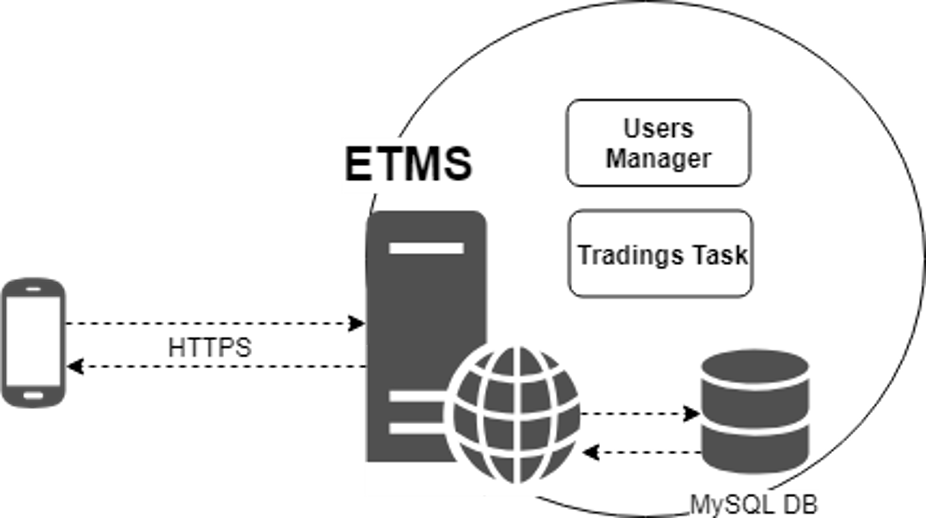
\includegraphics[width=0.9\textwidth]{./Images/ps12}
\caption{Power Share \ac{ETMS} architecture}
\label{fig:ps12}
\end{figure}

%%%%%%%%%%%%%%%% REFER ATTACHMENTS %%%%%%%%%%%%%%%
The Users Manager layer contains all the endpoints (\cref{chapter:appendixA}) available for an authenticated client. The authentication scheme used is Bearer Authentication, that is part of OAUTH 2.0\footnote{Authorization protocol that gives an \ac{API} client limited access to user data on a web server.} in RFC 6750\footnote{\url{https://tools.ietf.org/html/rfc6750}}. This Bearer token is generated on the login request and has to be used by the client in the “Authorization header” for all endpoints (except login and register). The \ac{API} requests used to feed the client application are GET, POST, UPDATE and DELETE. The full \ac{UML} database schema, with all parameters of each table and respective relations, can be found in \cref{chapter:appendixB}. From now on, any reference to a database table can be founded in that schema. 


A trading is the combination of three main asynchronous tasks. “Start transactions” (\cref{fig:ps13}), “Verify transactions” and “Stop Transactions” (\cref{fig:ps15}).

\textbf{Start Transactions:} Once a user has set his parameters for trading energy and activated the trading by sliding the switch to the on position, an entry with user id and sales/bough settings id are added in the database (in want\_sell or want\_buy table respectively). Such a combination of user id/settings id is unique. When the user starts a transaction or turns off the trading switch, this entry is removed from the table. Each minute the system verifies if there are entries in the want\_sell table and, for each entry found, the server runs the match algorithm to find a buyer whose demand for energy matches the seller settings - e.g. a seller that offers solar energy to neighbours at the same price (s)he pays energy to \ac{EEM} (let’s imagine, (s)he has “simples” tariff thus pays always 0,1629 € per kWh) will match and thus being able to trade with a consumer who has selected a maximum buying price that is equal or higher than 0,1629€/kWh. 

\begin{figure}[h]
\centering
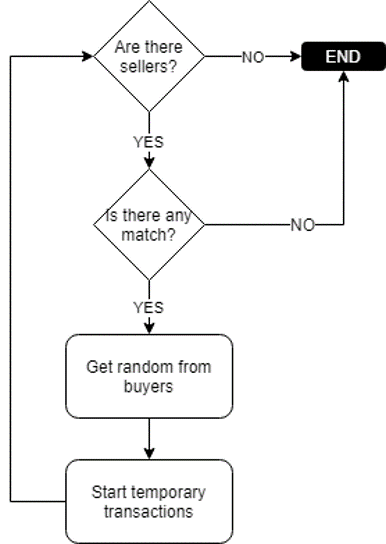
\includegraphics[width=0.4\textwidth]{./Images/ps13}
\caption{Start Transactions flow chart}
\label{fig:ps13}
\end{figure}

So, by selecting a specific selling price, sellers are guaranteed they will always sell energy for neither more nor less than that price. On the contrary, buyers cannot know in advance the actual amount they will pay for kWh. They are only guaranteed it will never be higher than the one they have set. In order to ensure impartiality, both sellers and matching buyers lists are shuffled. Every time the system finds a match, a temporary transaction is created, while the fields corresponding to the amount of energy consumed (by the buyer)  and remaining surplus (of the seller) are updated in the database. The transaction duration is configurable, however, we set one hour as a fixed time to perform each transaction. This choice was made after the analysis of historical consumption and production data of our users which lead us to conclude that, in less than one hour, the amount of energy exchanged could easily be so low  that the rounded value presented to the users is likely to be zero. 





\textbf{Verify transactions:} A possible scenario is that a seller has the trading on but no energy stored in the battery to sell. For this reason, every two minutes the system runs a verification transactions task (\cref{fig:ps14}). By performing this task, it verifies if the consumed energy in a temporary transaction is greater than zero (the system only verifies transactions running over five minutes). In case the value of a transaction is not higher than zero, it will be immediately stopped. The respective entry in the temporary\_transactions table is deleted and want\_buy and want\_sell tables are again updated.


\begin{figure}[h]
\centering
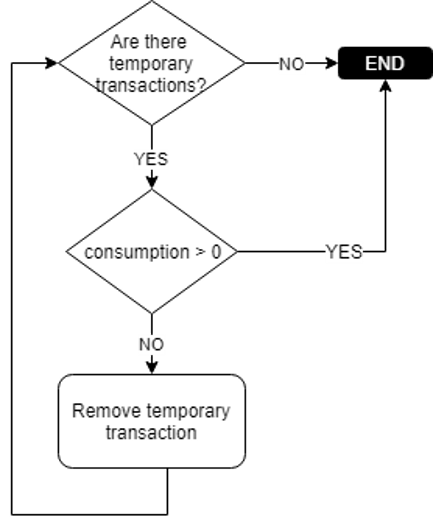
\includegraphics[width=0.4\textwidth]{./Images/ps14}
\caption{Verify Transactions flow chart}
\label{fig:ps14}
\end{figure}


\textbf{Stop Transactions:} This task consists in stopping all transactions with the duration equal to one hour. When a transaction ends, the system verifies if the energy actually used  by the buyer corresponds to the requested amount. In other words, the system verifies if the surplus energy made available by the seller is enough to meet the demand from the buyer and, in case it is not, updates the actual amount of energy traded accordingly. This can be done only at the end of the transaction due to concurrency restrictions, i.e. it is not guaranteed to have data from the buyer and the seller’s meters at the same time. The system is designed to not  stop any transaction if data is missing. In case the connection between the server and the smart meter should fail, the transaction won’t be stopped, i.e. none transactions is stopped if the last timestamp received by the buyer and/or seller’s meter is earlier than the end of the transaction (\cref{fig:ps15}). This is possible because the smart meter sends the data points sequentially.



\begin{figure}[h]
\centering
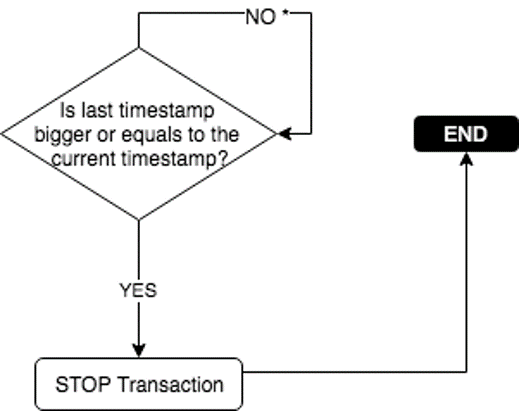
\includegraphics[width=0.4\textwidth]{./Images/ps15}
\caption{Stop Transactions flow chart}
\label{fig:ps15}
\end{figure}


At the end of each transaction, the system verifies if the seller has any available address for it and, if so, it associates the address with that transaction (\cref{fig:ps16}). If no address is available an asynchronous routine named \textbf{Transactions Addresses} task will be performed. This routine runs one time a day. It basically verifies if there are sales without an associated address and, in case it finds some, it will notify the respective users (sellers only) the need to generate new addresses for getting paid. This alert consists in an email and a push notification received directly on the mobile device where the app is installed.  



\begin{figure}[h]
\centering
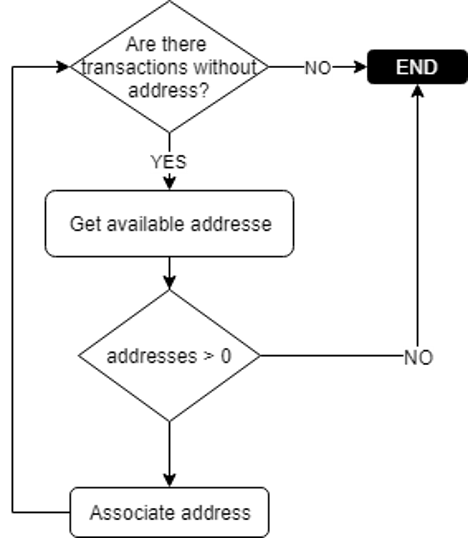
\includegraphics[width=0.4\textwidth]{./Images/ps16}
\caption{Transactions Addresses flow chart}
\label{fig:ps16}
\end{figure}

\subsection{Battery Simulation}

Technically, to trade energy by using this system, a prosumer does not need to have a \ac{BESS} (i.e. in the moment there is excess production and if there is demand, the the energy surplus can be sold in real time). However, having a \ac{BESS} will exponentially increase the effectiveness of this system, since users can store the energy surplus throughout the day and sell or use it later. For this reason, and since none of the participants in the field test have a battery, for the purpose of this study the system will simulate a 3000w “virtual battery” for each of them. Before explaining how this simulation is done, the following  information about a Battery Energy Storage System need to be provided:
\begin{itemize}
    \item The battery capacity represents the amount of energy that it can store (in kWh). Capacity is different from the power rating, which on the contrary represents the amount of energy (kW) a battery can provide in a given time frame.
    \item The \ac{DOD} defines the degree to which a battery is discharged in relation to its total capacity . In order to not compromise the battery lifetime, it should never reach 100\% or 0\% (the optimal \ac{DOD} should range between 20\% and 80\%). For the purpose of our study, in order to simplify the server logic we did not set a maximum and minimum \ac{DOD} for our “virtual batteries”;
    \item Batteries consume energy too. The \ac{RTE} is the term used to describe how much of the energy stored in the battery is lost in a “round trip” between the time the energy storage system is charged and then discharged \cite{energymag}. The \ac{RTE} of our virtual batteries is 80\% (i.e. 20\% of the energy stored is lost).
\end{itemize}

In this respect, in order to faithfully simulate the behaviour of an actual battery, the system  multiplies the amount of energy stored in the virtual battery by its \ac{RTE} (i.e. energy stored x 0,8), so to get the amount of energy available for trading. No losses are calculated on the amount of energy sold.
% #############################################################################
\section{IOTA integration} \label{ii}
Blockchain technology, more precisely IOTA, is used here as a payment system. For this purpose, \ac{IRI} was run on a Ubuntu 16.04.4 server equipped with a 6 cores processor and 8GB RAM.



Each node on the Tangle runs \ac{IRI} and needs other neighbours (i.e. other nodes running \ac{IRI}, which can be found on the official IOTA discord channel\footnote{\url{https://discordapp.com/invite/rYA7gFa}}) to perform a transaction.  Our node has three neighbors. In other words, the Tangle works as follow: one node performs a transaction and pays for it by validating two other non-validated transactions, called Tips, following the “Tip Selection” process. In order to validate the Tips \ac{IRI} issues the Tip Selection Algorithm Deep Dive that “has to walk a portion of the Tangle (subgraph) twice, stepping according to a rating calculation, selecting an entry point for each walk.”\cite{iotatips}. Since a user has to validate two transactions to get his one approved an efficient network is required, therefore the more active users in the network the better. In addition, it must be pointed out that, in order to perform the tips validation properly, neighbors need to be synchronized with the Tangle, run over a good machine (i.e. a powerful computer that, according with IOTA recommendations, should be at least equipped with a 2 cores processor and 4GB RAM) and have a stable network of neighbors in their turn. For this reason, we only know if a node is good or not by adding it as a neighbour and testing the network behavior. 


This way we can perform transactions using the Tangle through the IOTA \ac{API}, having a decentralized network operated by the Tangle that validates transactions between neighbors. Despite there are many public nodes available, we decide to run our own node since, if a public node becomes unstable, we don't have the possibility to fix it and consequently cannot guarantee the transaction will be performed successfully.  \ac{PS} relies on this node to perform the payments and the \ac{POW} is done as a service by the application. The POW on the Tangles is simpler compared to, for instance, the Bitcoin \ac{POW}, therefore it requires less computational power.



The energy traded is paid through IOTA cryptocurrency (MIOTA). For the purpose of our study, a given amount of MIOTA (around 10€) has been pre-purchased for each participant. It is then their responsibility to verify that the balance in their iota account is enough to keep trading. If the user runs out of MIOTA, the system will automatically disable the trading. 


As explained before, in order to get paid for the energy sold, the user needs to generate an address and it is his/her responsibility to do so. On the Tangle, one address could receive funds more than once, however, since we sent a transaction with specific address as input, we should never use that address again. Indeed, IOTA uses winternitz one-time signatures, which degrade security exponentially after each use of the same address \cite{iotaseeds}.



